\documentclass{beamer}
\usepackage[french]{babel}
\usepackage{hyperref}
\usepackage{graphicx}
\usepackage{amsmath,amssymb}
\usepackage{tabularx}
\usepackage{booktabs}
\usepackage[compatibility=false]{caption}
\usepackage[toc,page]{appendix}
\usepackage{minted}
\usepackage{xspace}
\usepackage{fourier}

\setminted{autogobble}

\setbeamercovered{transparent}
%\makeatletter
%  \def\beamer@calltheme#1#2#3{%
%    \def\beamer@themelist{#2}
%    \@for\beamer@themename:=\beamer@themelist\do
%    {\usepackage[{#1}]{\beamer@themelocation/#3\beamer@themename}}}
%
%  \def\usefolder#1{
%    \def\beamer@themelocation{#1}
%  }
%  \def\beamer@themelocation{}
%
%\patchcmd{\minted@colorbg}{\noindent}{\medskip\noindent}{}{}
%\apptocmd{\endminted@colorbg}{\par\medskip}{}{}
%\makeatother

\newcolumntype{Y}{>{\centering\arraybackslash}X}

%\usefolder{../theme}
\usetheme[numbering=fraction,block=fill,progressbar=frametitle]{metropolis} %Use metropolis theme
%\usetheme{CambridgeUS} %Use Cambridge theme

\definecolor{bg}{rgb}{0.95,0.95,0.95}
\setminted{bgcolor=bg,fontsize=\scriptsize,autogobble,mathescape,breaklines,tabsize=2}
\setmintedinline{breaklines,autogobble,fontsize=\scriptsize}
\setbeamersize{text margin left=8pt,text margin right=8pt}

\begin{document}

\title[Cours d'algorithmique]{Algorithmique et structures de données}
\author[nicolas.audebert@lecnam.net]{Nicolas Audebert}
\setmainfont{Fira Sans}


\AtBeginSection[]{
  \begin{frame}{Plan de la séance}
  \small \tableofcontents[currentsection]
  \end{frame}
}

\date[7 mars 2022]{Lundi 7 mars 2022}
\subtitle{File de priorité - Fast marching}
\maketitle

\section{File de priorité et tri par tas}

\begin{frame}{File de priorité}
L'objectif est de créer une file dont les éléments sont retirés en fonction de la \textbf{priorité} (un score) qui leur est attribué.

Il s'agit donc de maintenir une file triée (par ordre de priorité) lors de l'ajout ou de la suppression d'un élément.

\begin{block}{Compromis}
  \begin{itemize}
  \item Accéder en $O(1)$, implique une insertion en $O(N)$
  \item Insérer en $O(1)$, implique un accès en $O(N)$
  \end{itemize}
\end{block}

\end{frame}

\begin{frame}{File de priorité : solution}
\begin{alertblock}{Solution}
  On fait le choix d'une insertion et d'un accès en $O(\log N)$. On utilise pour ce faire une structure d'\textbf{arbre binaire} équilibré, i.e. un arbre dans lequel chaque noeud possède au plus 2 fils. On construit l'arbre de sorte que chaque parent a une priorité supérieure à celle de ses fils.
\end{alertblock}
\end{frame}

\begin{frame}{File de priorité : insertion (push)}

Le nouvel élément est inséré dans le sous-arbre de profondeur minimale, puis échangé avec ses parents si sa priorité est supérieur à la leur.

\begin{figure}
\centering
\includegraphics<1>[width = 0.4\linewidth]{./images/heap_push1.pdf}
\includegraphics<2>[width = 0.4\linewidth]{./images/heap_push2.pdf}
\includegraphics<3>[width = 0.4\linewidth]{./images/heap_push3.pdf}
\includegraphics<4>[width = 0.4\linewidth]{./images/heap_push4.pdf}
\includegraphics<5>[width = 0.4\linewidth]{./images/heap_push5.pdf}
\end{figure}
\end{frame}

\begin{frame}{File de priorité : retrait (pop)}
La racine de l'arbre est retirée. L'élément le plus profond est placé à la racine puis échangé avec son fils de priorité maximale si celle-ci est supérieure à la sienne. 

\begin{figure}
\centering
\includegraphics<1>[width = 0.4\linewidth]{./images/heap_pop1.pdf}
\includegraphics<2>[width = 0.4\linewidth]{./images/heap_pop2.pdf}
\includegraphics<3>[width = 0.4\linewidth]{./images/heap_pop3.pdf}
\includegraphics<4>[width = 0.4\linewidth]{./images/heap_pop4.pdf}
\includegraphics<5>[width = 0.4\linewidth]{./images/heap_pop5.pdf}
\includegraphics<6>[width = 0.4\linewidth]{./images/heap_pop6.pdf}
\includegraphics<7>[width = 0.4\linewidth]{./images/heap_pop7.pdf}
\end{figure}
\end{frame}

\begin{frame}{Stockage}
La file de priorité est stockée dans un tableau, construit de la façon suivante\,:

En commençant à l'indice 1, les fils du n{\oe}ud $i$ sont placés aux indices $2i$ et $2i+1$.

\vspace{1cm}
\includegraphics<1>[width=\linewidth]{images/stockage1.pdf} 
\includegraphics<2>[width=\linewidth]{images/stockage2.pdf} 
\includegraphics<3>[width=\linewidth]{images/stockage3.pdf} 
\includegraphics<4>[width=\linewidth]{images/stockage4.pdf} 
\end{frame}

\section{Tri par tas}
\begin{frame}[fragile]{HeapSort}

\textbf{HeapSort} remplit une file de priorité et puis retire les éléments un par un.
\begin{minted}{cpp}
void HeapSort(std::vector<double> &v){
  FilePriorite f;
  for(int i=0; i<v.size(); i++){
    f.push(v[i]);
  }
  for(int i=0; i<v.size(); i++){
    v[i] = f.pop();
  }
}
\end{minted}
\end{frame}

\begin{frame}{Conclusion}
HeapSort est un tri en $O(N \log N)$ \textbf{dans tous les cas}. Cependant en comparaison à QuickSort, il utilise plus de mémoire et est plus long en moyenne.

En pratique, QuickSort est le tri le plus utilisé.
\end{frame}


\begin{frame}{Complexités à retenir}

\begin{itemize}
\item Tri : $O(N \log N)$
\item Recherche dans un tableau trié : $O(\log N)$
\item Recherche dans un tableau non trié : $O(N)$
\end{itemize}

\end{frame}

\section{TP}

\begin{frame}{TP : fast marching}

\begin{block}{TP}
Deux parties :
\begin{itemize}
\item Implémentation d'une file de priorité
\item Application au fast marching
\end{itemize}
\end{block}
\end{frame}

\begin{frame}{Fast marching}

\begin{block}{Calcul rapide de cartes de distances}
\centering

\vspace{1cm}
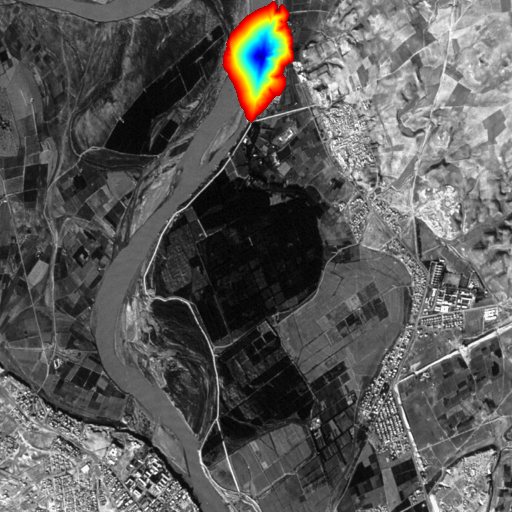
\includegraphics[width=0.4\linewidth]{images/road2-propagation-005.png}~~~

\includegraphics[width=0.4\linewidth]{images/road2-propagation-013.png}
\end{block}
\end{frame}

\begin{frame}{Fast marching}

\begin{block}{Calcul de plus court chemin}
\centering


\begin{minipage}{0.45\linewidth}

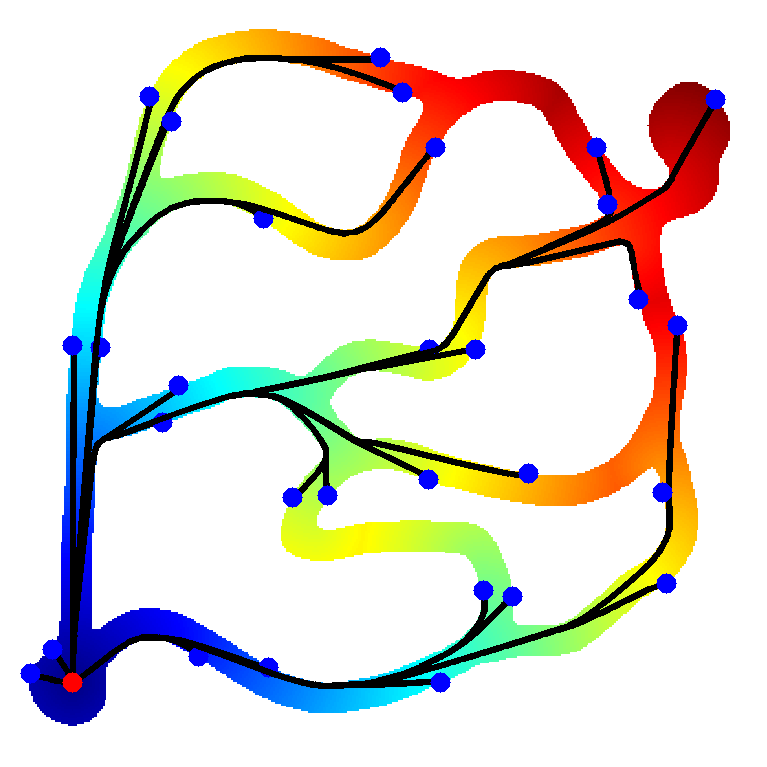
\includegraphics[width=\linewidth]{images/cavern-geodesics.png}
\end{minipage}
~~~
\begin{minipage}{0.45\linewidth}
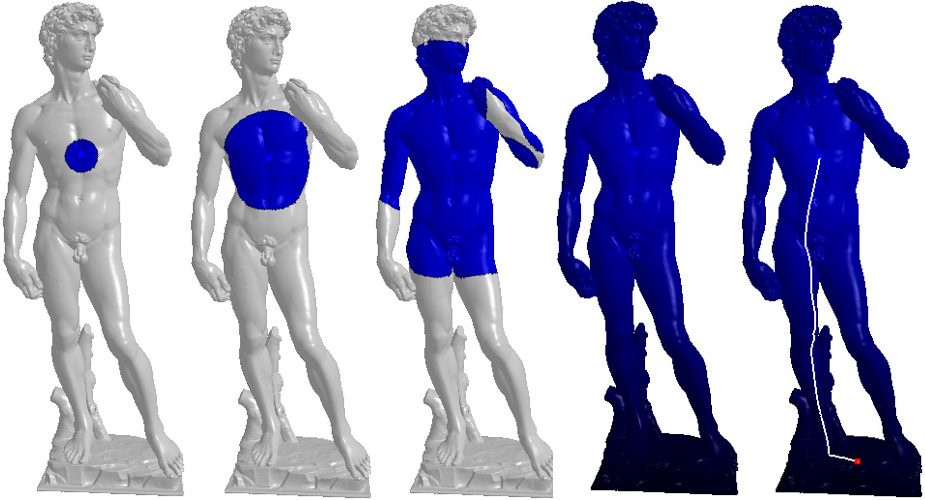
\includegraphics[width=\linewidth]{images/test_geodesic.jpg}

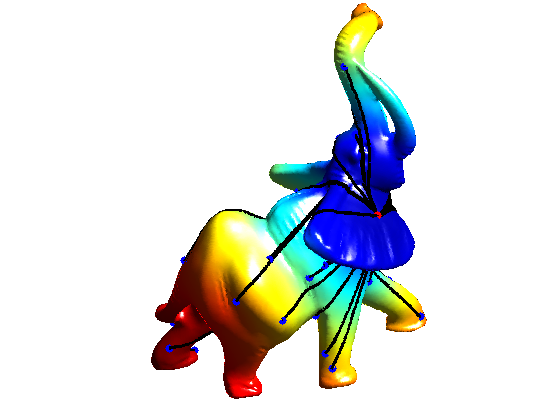
\includegraphics[width=\linewidth]{images/content_08.png}
\end{minipage}
\end{block}

\end{frame}

% \begin{frame}{Google Code Jam}
% 
\includegraphics[width=\linewidth]{images/Code-Jam-2015.jpg}
% \begin{itemize}
% \item Concours de code international
% \item Problèmes d'algorithmie
% \item Petit et gros dataset
% \item Inscription à partir d'aujourd'hui, début en avril
% \end{itemize}
% \end{frame}
% 
% \begin{frame}{Exercice : Google Code Jam 2010}
% \begin{block}{Problem}
% You receive a credit C at a local store and would like to buy two items. You first walk through the store and create a list L of all available items. From this list you would like to buy two items that add up to the entire value of the credit. The solution you provide will consist of the two integers indicating the positions of the items in your list (smaller number first).
% \end{block}
% \end{frame}
% 
% \begin{frame}[fragile]{Exercice : Google Code Jam 2010}
% 
% \begin{minipage}{0.48\linewidth}
% \begin{lstlisting}
% Input 
% 
% 3
% 100
% 3
% 5 75 25
% 200
% 7
% 150 24 79 50 88 345 3
% 8
% 8
% 2 1 9 4 4 56 90 3
% \end{lstlisting}
% \end{minipage}
% \hfill
% \begin{minipage}{0.48\linewidth}
% \begin{lstlisting}
% Output 
% 
% Case #1: 2 3
% Case #2: 1 4
% Case #3: 4 5
% \end{lstlisting}
% \end{minipage}
% \end{frame}
% 
% \begin{frame}{Solution}
% 
% Tester toutes les paires.
% 
% \begin{alertblock}{Solution naïve}
% Solution en $O(N^2)$.
% Risque de ne pas être efficace pour le gros dataset.
% \end{alertblock}
% 
% \end{frame}
% 
% \begin{frame}[fragile]{Solution 2}
% 
% \begin{CppBlock}
% \begin{lstlisting}
% // charger les donnees du fichier
% int S = ... // la somme
% vector<int> articles = ...
% 
% // trier la liste des indices en fonction des prix
% vector<int> id_tries = ...
% 
% // rechercher la paire dans un ensemble trie
% int i=0, j=id_tries.size()-1;
% while(i<j){
%   if(article[id_tries[i]]+article[id_tries[j]]== S)
%   	break;
%   if(article[id_tries[i]]+article[id_tries[j]] < S)
%   	i++;
%   if(article[id_tries[i]]+article[id_tries[j]] > S)
%   	j--;
% }
% 
% // ecrire la solution
% \end{lstlisting}
% \end{CppBlock}
% 
% Solution en $O(N\, \log\, N)$
% 
% \end{frame}
\end{document}
